\documentclass{article}
\usepackage[utf8]{inputenc}

\usepackage{amsmath}
\usepackage{courier}
\usepackage[margin=1in]{geometry}
\usepackage{graphicx}
\usepackage{hyperref}
\usepackage{listings}
\usepackage{subcaption}
\usepackage{microtype}
\usepackage{mathtools}
\usepackage{amssymb}
\usepackage{cleveref}
\usepackage{tabularx}

\hypersetup{
    colorlinks=true,
    urlcolor=blue,
}

\lstset{basicstyle=\footnotesize\ttfamily, breaklines=true}

\title{Assignment 1: Convolution and Hybrid Images}
\author{CS 4476}
\date{Spring 2024}

\begin{document}

\maketitle

\section*{Logistics}
\begin{itemize}
    \item Due: 23:59 January 28th EST (Check course syllabus for late policy)
    % \item{Assignment materials including report template: \href{}{Project 1}}
    \item{Hand-in: \href{https://www.gradescope.com}{Gradescope}}
    \item{Required files: \lstinline{<your_gt_username>.zip}, \lstinline{<your_gt_username>_project1.pdf}}
\end{itemize}

\begin{figure}[htt]
    \centering
    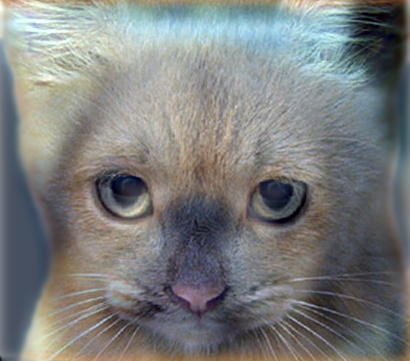
\includegraphics[width=0.5\textwidth]{images/hybrid_image.jpg}
    \caption{Look at the image from very close, then from far away.}
    \label{fig:hybrid}
\end{figure}


\section*{Overview}
The goal of this assignment is to write an image filtering function and use it to create hybrid images using a simplified version of the SIGGRAPH 2006 \href{http://olivalab.mit.edu/publications/OlivaTorralb_Hybrid_Siggraph06.pdf}{paper} by Oliva, Torralba, and Schyns. \textit{Hybrid images} are static images that change in interpretation as a function of the viewing distance. The basic idea is that high frequency tends to dominate perception when it is available but, at a distance, only the low frequency (smooth) part of the signal can be seen. By blending the high frequency portion of one image with the low-frequency portion of another, you get a hybrid image that leads to different interpretations at different distances.
\\
\\
This project is intended to familiarize you with \lstinline{Python}, \lstinline{PyTorch}, and image filtering. Once you have created an image filtering function, it is relatively straightforward to construct hybrid images. If you don't already know Python, you may find \href{https://docs.python.org/3/tutorial/}{this resource} helpful. If you are more familiar with MATLAB, \href{http://mathesaurus.sourceforge.net/matlab-numpy.html}{this guide} is very helpful. If you're unfamiliar with PyTorch, the \href{https://pytorch.org/tutorials/}{tutorials} from the official website are useful. \textit{However, all assignments in this course need to be completed using Python.}


\section*{Setup}
\begin{enumerate}
    \item Check Assignment 0 for environment installation.
    \item Run the notebook using \lstinline{jupyter notebook ./project-1.ipynb} or other IDEs that support jupyter notebook.
    \item After implementing all functions, ensure that all sanity checks are passing by running \lstinline{pytest tests} inside the main folder.
    \item Generate the zip folder for the code portion of your submission once you've finished the project using \lstinline{python zip_submission.py --gt_username <your_gt_username>}
\end{enumerate}

\section*{Rubric (100 pts in total)}

\paragraph{80 pts: Coding}
\begin{itemize}
    \setlength\itemsep{-0.3em}
    \item 5 pts: \lstinline{create_Gaussian_kernel_1D()} in \lstinline{part1.py}
    \item 5 pts: \lstinline{create_Gaussian_kernel_2D()} in \lstinline{part1.py}
    \item 5 pts: \lstinline{separate_Gaussian_kernel_2D()} in \lstinline{part1.py}
    \item 12.5 pts: \lstinline{my_conv2d_numpy()} in \lstinline{part1.py}
    \item 7.5 pts: \lstinline{create_hybrid_image()} in \lstinline{part1.py}
    \item 5 pts: \lstinline{make_dataset()} in \lstinline{part2_datasets.py}
    \item 5 pts: \lstinline{get_cutoff_frequencies()} in \lstinline{part2_datasets.py}
    \item 5 pts: \lstinline{__len__()} in \lstinline{part2_datasets.py}
    \item 5 pts: \lstinline{__getitem__()} in \lstinline{part2_datasets.py}
    \item 5 pts: \lstinline{get_kernel()} in \lstinline{part2_models.py}
    \item 5 pts: \lstinline{low_pass()} in \lstinline{part2_models.py}
    \item 10 pts: \lstinline{forward()} in \lstinline{part2_models.py}
    \item 5 pts: \lstinline{my_conv2d_pytorch()} in \lstinline{part3.py}
\end{itemize}
\paragraph{20 pts: Writeup Report}
\begin{itemize}
    \setlength\itemsep{-0.3em}
    \item 1 pts: page 2 (Part 1: Gaussian Kernels)
    \item 1 pts: page 3 (Part 1: Image filtering)
    \item 1 pts: page 4 (Part 1: Image filtering)
    \item 1 pts: page 5 (Part 1: Image filtering)
    \item 1.5 pts: page 6 (Part 1: Hybrid images)
    \item 1.5 pts: page 7 (Part 1: Hybrid images)
    \item 1.5 pts: page 8 (Part 1: Hybrid images)
    \item 1.5 pts: page 9 (Part 2: Hybrid images with PyTorch)
    \item 1.5 pts: page 10 (Part 2: Hybrid images with PyTorch)
    \item 1.5 pts: page 11 (Part 2: Hybrid images with PyTorch)
    \item 2 pts: page 12 (Part 3: Understanding input/output shapes in PyTorch)
    \item 1 pts: page 13 (Part 3: Understanding input/output shapes in PyTorch)
    \item 1 pts: page 14 (Part 3: Understanding input/output shapes in PyTorch)
    \item 1 pts: page 15 (Part 3: Understanding input/output shapes in PyTorch)
    \item 1 pts: page 16 (Part 3: Understanding input/output shapes in PyTorch)
    \item 1 pts: page 17 (Conclusion)
\end{itemize}
(-5*n pts: Lose 5 points for every time you do not follow the instructions for the hand-in format)


\section{NumPy}

\subsection{Gaussian Kernels}

\paragraph{Univariate Gaussian Kernels.}
Gaussian filters are used for blurring images. You will first implement \lstinline{create_Gaussian_kernel_1D()}, a function that creates a 1D Gaussian vector according to two parameters: the kernel size (length of the 1D vector) and $\sigma$, the standard deviation of the Gaussian. The vector should have values populated from evaluating the 1D Gaussian probability density function (pdf) at each coordinate. The 1D Gaussian pdf is defined as:
\begin{align}
f_X(x; \mu, \sigma^2) \triangleq \frac{1}{\sqrt{2\pi} \sigma} \exp \left( -\frac{1}{2\sigma^2}(x - \mu)^2 \right)
\end{align}

\paragraph{Multivariate Gaussian Kernels.} 
Next, you will implement \lstinline{create_Gaussian_kernel_2D()}, which creates a 2-dimensional Gaussian kernel according to a free parameter, \textit{cutoff frequency}, which controls how much low frequency to leave in the image. Choosing an appropriate cutoff frequency value is an important step for later in the project when you create hybrid images. We recommend that you implement \lstinline{create_Gaussian_kernel_2D()} by creating a 2D Gaussian kernel as the outer product of two 1D Gaussians, which you have now already implemented in \lstinline{create_Gaussian_kernel_1D()}. This is possible because the 2D Gaussian filter is \emph{separable} (think about how $e^{(x+y)} = e^x \cdot e^y$). The multivariate Gaussian function is defined as:
\begin{align}
    f_{\boldsymbol{X}}(\boldsymbol{x}; \boldsymbol{\mu}, \boldsymbol{\Sigma}) &\triangleq \frac{1}{Z} \exp\left(-\frac{1}{2}(x - \boldsymbol{\mu})^\top \boldsymbol{\Sigma}^{-1} (x - \boldsymbol{\mu})\right) \label{eqn:normal} \\ 
    \shortintertext{where \(\boldsymbol{\mu} \in \mathbb{R}^2\) is the mean vector, \(\boldsymbol{\Sigma} \in \mathbb{R}^{2 \times 2}\) is the covariance, and \(Z\) is the normalization constant:}
    Z &\triangleq \frac{1}{(2\pi)^{n / 2} \det(\boldsymbol{\Sigma})^{1 / 2}}
\end{align}
\paragraph{Properties of Gaussian Kernels.}
It is a fact that for the Gaussian pdf:
\begin{align}
    \boldsymbol{\mu} = \underset{\boldsymbol{x}}{\text{argmax }} f_{\boldsymbol{X}}\left(\boldsymbol{x}; \mu, \Sigma \right)
\end{align}
Indeed, for discrete Gaussian kernels which are indexed from \(0\) to \(k - 1\), it is the case that:
\(\boldsymbol{\mu} = \left( \lfloor \frac{k}{2} \rfloor, \lfloor \frac{k}{2} \rfloor, \dots, \lfloor \frac{k}{2} \rfloor \right) \) -- this is shown qualitatively in \cref{fig:gaussian-7x7}.
Additionally, we can see that \(Z\) is defined as such to ensure that the distribution in \cref{eqn:normal} satisfies the second axiom of probability:
\begin{align}
    \int_{-\infty}^{\infty} f_{\boldsymbol{X}}\left(\boldsymbol{x}; \boldsymbol{\mu}, \boldsymbol{\Sigma}\right) = 1
\end{align}
It should be noted that if your kernel (discrete) does not satisfy the above axiom, you should normalize it with:
\begin{align}
    Z = \sum_{i=0}^{k-1}\sum_{j=0}^{k-1} f_{\boldsymbol{X}}\left( (i, j); \boldsymbol{\mu}, \boldsymbol{\Sigma} \right)
\end{align}

\begin{figure}
    \centering
    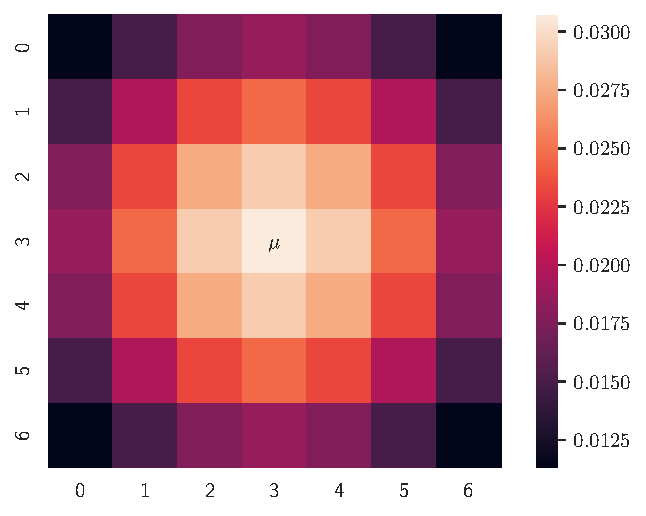
\includegraphics{gaussian-7x7.pdf}
    \caption{A \(7 \times 7 \) Gaussian kernel with \(\boldsymbol{\mu} = (\lfloor \frac{7}{2} \rfloor, \lfloor \frac{7}{2} \rfloor)\) and \(\boldsymbol{\Sigma} = I\).}
    \label{fig:gaussian-7x7}
\end{figure}

\paragraph{Separable Kernels.} In many cases, the filtering operation can be significantly sped up by first performing a one-dimensional horizontal filtering followed by a one-dimensional vertical filtering. A filtering kernel for which this is possible is said to be separable. As mentioned above, 2D Gaussian kernels are separable kernels. See chapter 3.2.1 of Szeliski to learn about the detailed explanation and process of kernel separation. You will implement \lstinline{separate_Gaussian_kernel_2D()}, which will separate an input 2D Gaussian kernel into two 1D kernels using Singular Value Decomposition(SVD) that fulfill the following equation:
\begin{align}
    \mathbf{K} = \mathbf{v} \mathbf{h}^T
\end{align}
\noindent
where $\mathbf{K}$ is the original 2D kernel, and $\mathbf{v}$ and $\mathbf{h}$ are the separated vertical and horizontal kernels.
\\
\noindent
The separated kernels can be achieved with the following:
\begin{align}
    \mathbf{v} = \sqrt{\mathbf{S}_0} \mathbf{U}_0 \\
    \mathbf{h}^T = \sqrt{\mathbf{S}_0} \mathbf{V_h}_0^T
\end{align}
\noindent
where $\mathbf{U}, \mathbf{S}, \mathbf{V_h}$ are the results of SVD (The symbols are changed for easier coding and different from Szeliski).
\\
\\
\noindent
After implementing the function, explain why separated kernels can speed up the filtering operations in several sentences briefly.

\subsection{Image Filtering}
Image filtering (or convolution) is a fundamental image processing tool. See chapter 3.2 of Szeliski and the lecture materials to learn about image filtering (specifically linear filtering). You will be writing your own function to implement image filtering from scratch. More specifically, you will implement \lstinline{my_conv2d_numpy()} which imitates the \lstinline{filter2D()} function in the OpenCV library. As specified in \lstinline{part1.py}, your filtering algorithm must: (1) support grayscale and color images, (2) support arbitrarily-shaped filters, as long as both dimensions are odd (e.g., $7\times9$ filters, but not $4\times5$ filters), (3) pad the input image with zeros, and (4) return a filtered image which is the same resolution as the input image. We have provided an iPython notebook, \lstinline{project-1.ipynb} and some unit tests (which are called in the notebook) to help you debug your image filtering algorithm. Note that there is a time limit of 5 minutes for a single call to \lstinline{my_conv2d_numpy()}, so try to optimize your implementation if it goes over.

\subsection{Hybrid Images}
A hybrid image is the sum of a low-pass filtered version of one image and a high-pass filtered version of another image. As mentioned above, \textit{cutoff frequency} controls how much high frequency to leave in one image and how much low frequency to leave in the other image. In \lstinline{cutoff_frequencies.txt}, we provide a default value of 7 for each pair of images (the value of line $i$ corresponds to the cutoff frequency value for the $i$-th image pair). You should replace these values with the ones you find work best for each image pair. In the paper it is suggested to use two cutoff frequencies (one tuned for each image), and you are free to try that as well. In the starter code, the cutoff frequency is controlled by changing the standard deviation of the Gaussian filter used in constructing the hybrid images. You will first implement \lstinline{create_hybrid_image()} according to the starter code in \lstinline{part1.py}. Your function will call \lstinline{my_conv2d_numpy()} using the kernel generated from \lstinline{create_Gaussian_kernel()} to create low and high frequency images, and then combine them into a hybrid image.


\section{PyTorch}

\subsection{Dataloader}
You will now implement creating hybrid images again but using PyTorch. The \lstinline{HybridImageDataset} class in \lstinline{part2_datasets.py} will create tuples using pairs of images with a corresponding cutoff frequency (which you should have found from experimenting in Part 1). The image paths will be loaded from \lstinline{data/} using \lstinline{make_dataset()} and the cutoff frequencies from \lstinline{cutoff_frequencies.txt} using \lstinline{get_cutoff_frequencies()}. Additionally, you will implement \lstinline{__len__()}, which returns the number of image pairs, and \lstinline{__getitem__()}, which returns the \lstinline{i}-th tuple. Refer to \href{https://pytorch.org/tutorials/beginner/data_loading_tutorial.html}{this tutorial} for additional information on data loading \& processing.

\subsection{Model}
Next, you will implement the \lstinline{HybridImageModel} class in \lstinline{part2_models.py}. Instead of using your implementation of \lstinline{my_conv2d_numpy()} to get the low and high frequencies from a pair of images, \lstinline{low_pass()} should use the 2D convolution operator from \lstinline{torch.nn.functional} to apply a low pass filter to a given image. You will have to implement \lstinline{get_kernel()} which calls your \lstinline{create_Gaussian_kernel()} function from \lstinline{part1.py} for each pair of images using the cutoff frequencies as specified in \lstinline{cutoff_frequencies.txt}, and reshape it to the appropriate dimensions for PyTorch. Then, similar to \lstinline{create_hybrid_image()} from \lstinline{part1.py}, \lstinline{forward()} will call \lstinline{get_kernel()} and \lstinline{low_pass()} to create the low and high frequency images, and combine them into a hybrid image. Refer to \href{https://pytorch.org/tutorials/beginner/blitz/neural_networks_tutorial.html}{this tutorial} for additional information on defining neural networks using PyTorch.
\\
\\
You will compare the runtimes of your hybrid image implementations from Parts 1 \& 2.


\section{Understanding input/output shapes in PyTorch}
You will now implement \lstinline{my_conv2d_pytorch()} in \lstinline{part3.py} using the same 2D convolution operator from \lstinline{torch.nn.functional} used in \lstinline{low_pass()}.

Before we proceed, here are two quick definitions of terms we'll use often when describing convolution:
\begin{itemize}
    \item \textbf{Stride}: When the stride is 1 then we move the filters one pixel at a time. When the stride is 2 (or uncommonly 3 or more, though this is rare in practice) then the filters jump 2 pixels at a time as we slide them around. 
    \item \textbf{Padding}: The amount of pixels added to an image when it is being convolved with a the kernel. Padding can help prevent an image from shrinking during the convolution operation.
\end{itemize}

\noindent
Unlike \lstinline{my_conv2d_numpy()} from \lstinline{part1.py}, the shape of your output does not necessarily have to be the same as the input image. Instead, given an input image of shape $(1, d_1, h_1, w_1)$ and kernel of shape $(N, \frac{d_1}{g}, k, k)$, your output will be of shape $(1, d_2, h_2, w_2)$ where $g$ is the number of groups, $d_2 = N$, $h_2 = \frac{h_1 - k + 2 * p}{s} + 1$, and $w_2 = \frac{w_1 - k + 2 * p}{s} + 1$, and $p$ and $s$ are padding and stride, respectively. 
\\
\\
Think about \emph{why} the equations for output width $w_2$ and output height $h_2$ are true -- try sketching out a $5 \times 5$ grid, and seeing how many places you can place a $3 \times 3$ square within the grid with stride 1. What about with stride 2? Does your finding match what the equation states?
\\
\\
Going through the convolution process can help understand this whole process. Consider the following image $\mathbf{M}$ and kernel $\mathbf{K}$. They have been simplified to two matrices with a single channel for each.
\begin{table}[h]
  \centering
  $\mathbf{M} =$ 
  \begin{tabularx}{0.1\textwidth} { 
      | >{\centering\arraybackslash}X 
      | >{\centering\arraybackslash}X 
      | >{\centering\arraybackslash}X | }
     \hline
     4 & 4 & 7 \\
     \hline
     6 & 4 & 7 \\
     \hline
     6 & 4 & 4 \\
    \hline
\end{tabularx}
\end{table}
\begin{table}[h]
  \centering
  $\mathbf{K} = $
    \begin{tabularx}{0.09\textwidth} { 
      | >{\centering\arraybackslash}X 
      | >{\centering\arraybackslash}X | }
     \hline
     1 & 2 \\
     \hline
     -1 & 1 \\
    \hline
    \end{tabularx}
\end{table}
\noindent
Use the kernel $\mathbf{K}$ to filter through the image $\mathbf{M}$ with stride 1 and padding 1 for calculation simplicity by hand. For padding, simply append $0$s to each side of the image. Show the calculation process in the writeup. (Hint: Predict the filtered image shape with the equations given above first, and compare the predicted shape with the actual filtered image shape.)
\\
\\
We demonstrate the effect of the value of the \lstinline{groups} parameter on a simple example with an input image of shape $(1, 2, 3, 3)$ and a kernel of shape $(4, 1, 3, 3)$:

\begin{figure}[ht]
    \centering
    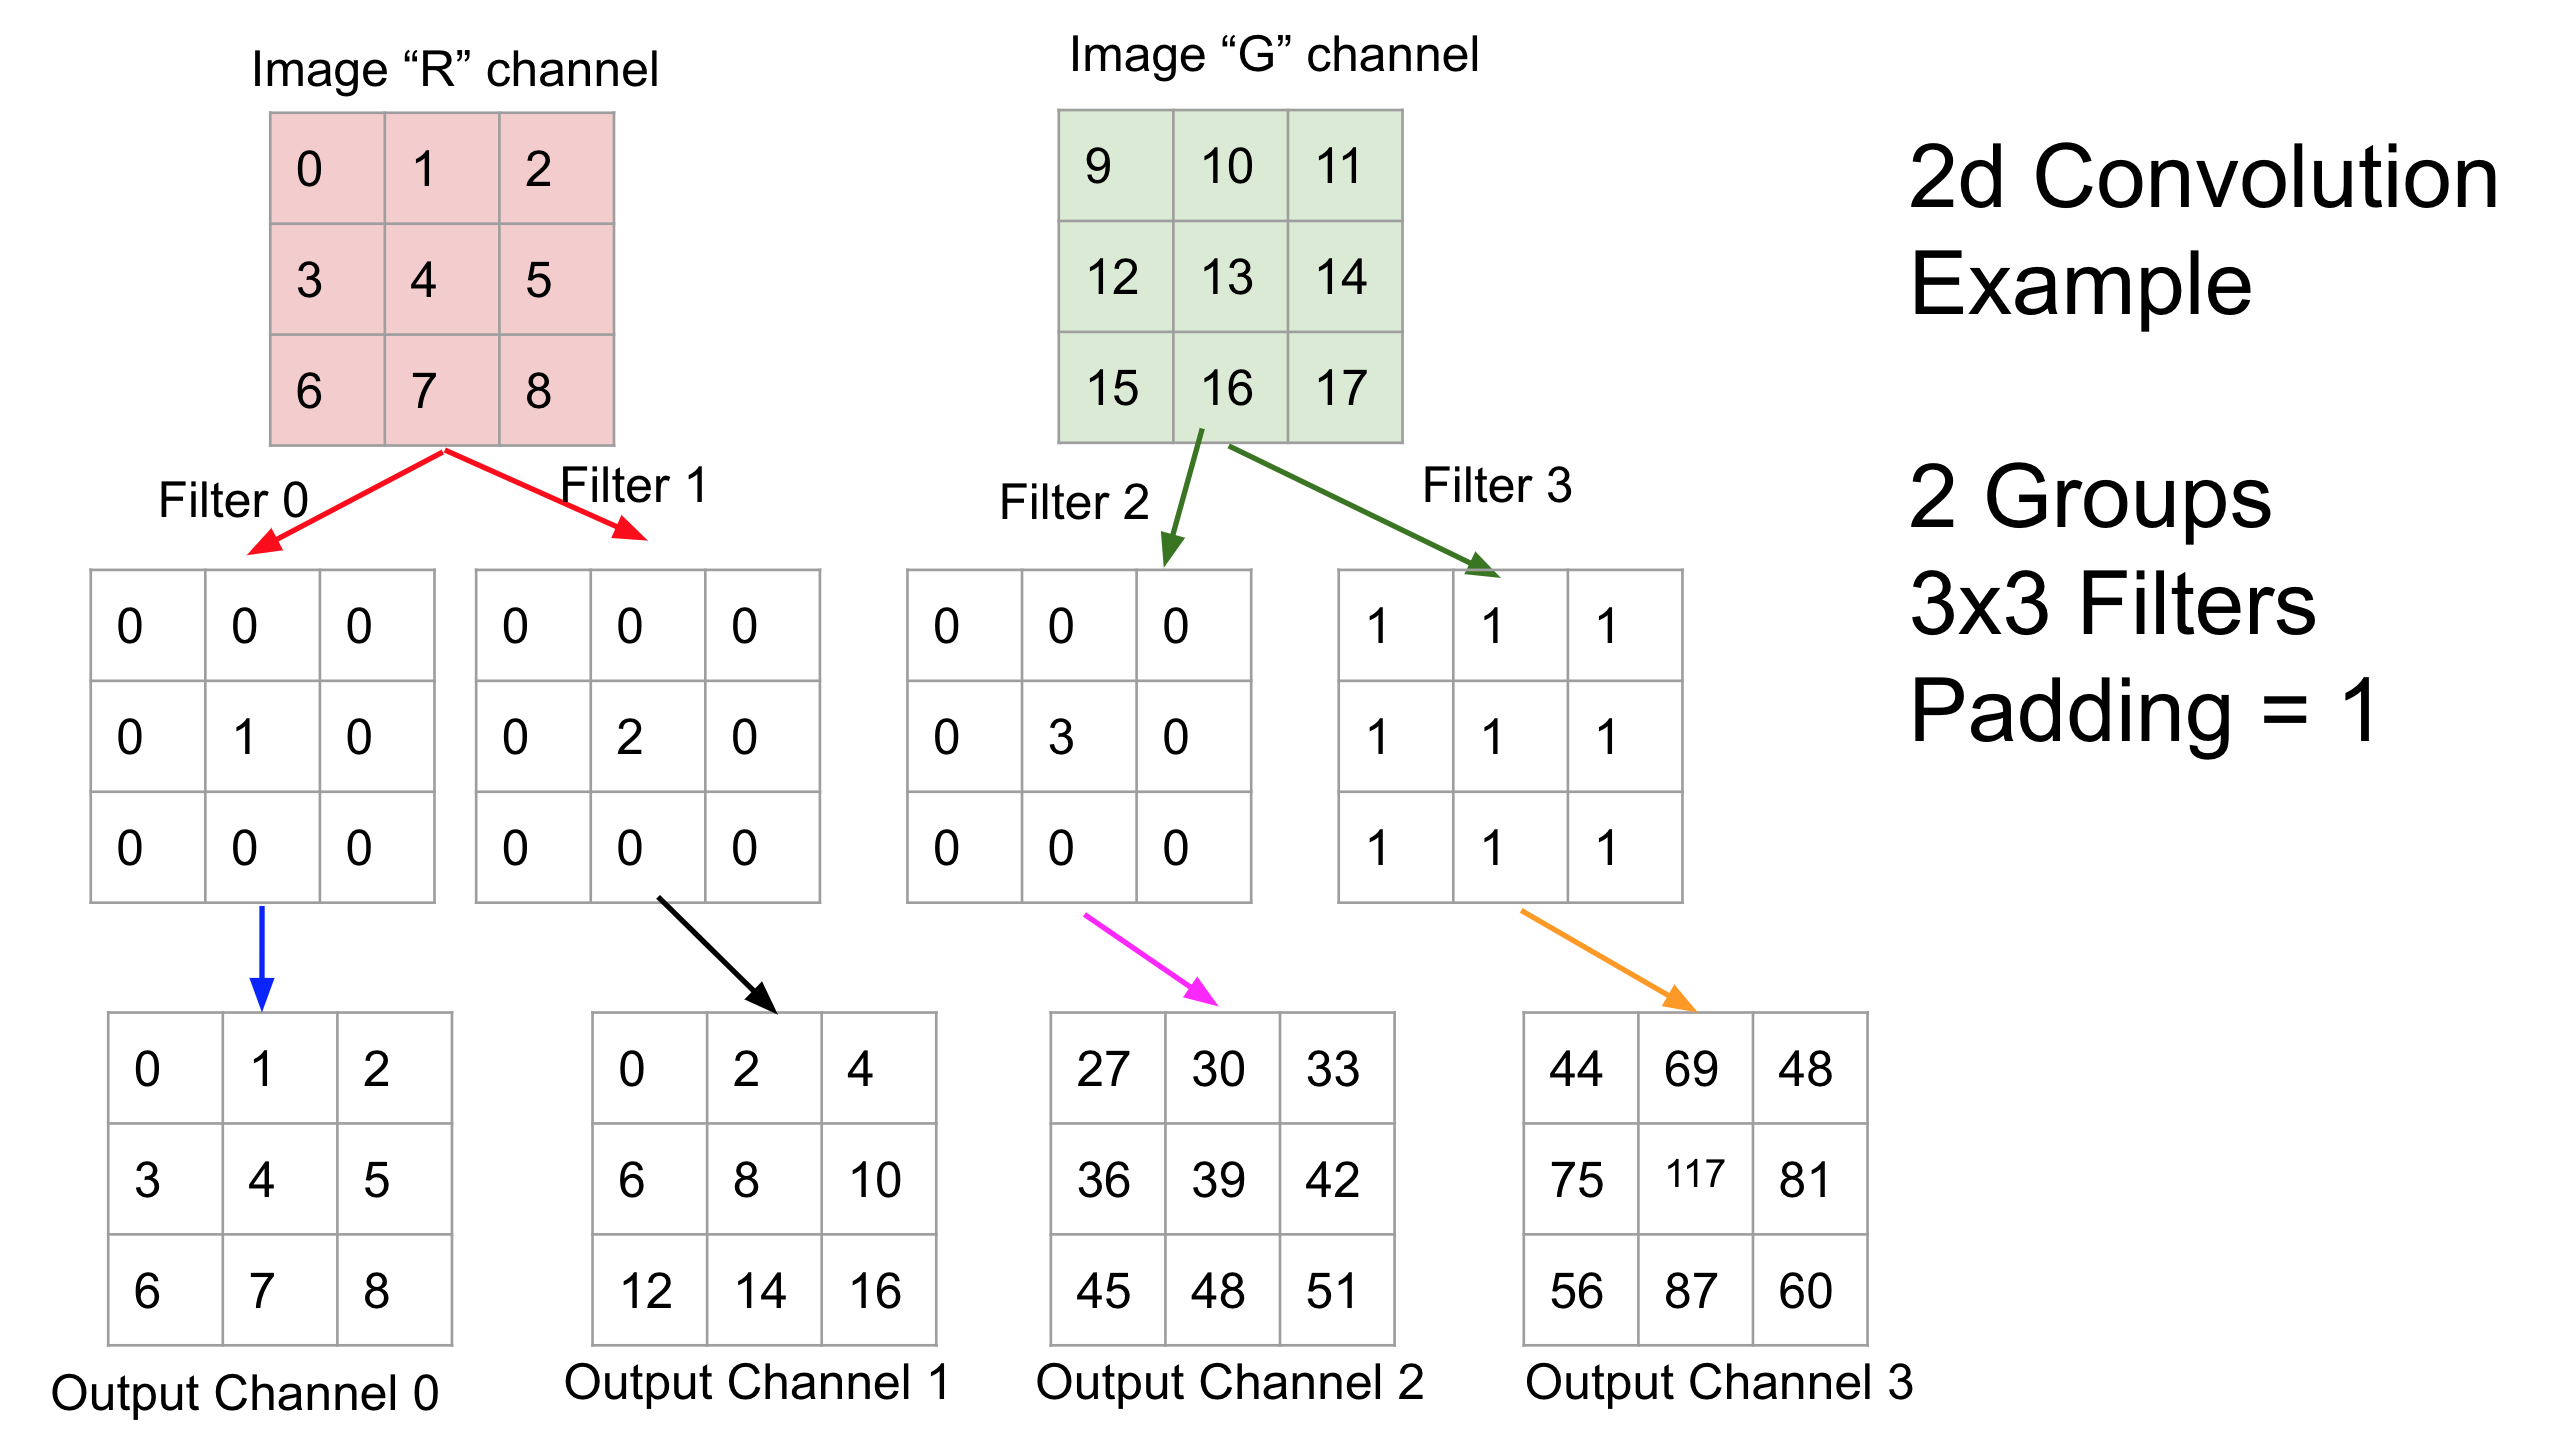
\includegraphics[width=0.75\textwidth]{images/part3_groups.png}
    \caption{Visualization of a simple example using \lstinline{groups=2}.}
    \label{fig:groups}
\end{figure}


\section{Writeup}
For this project (and all other projects), you must do a project report using the template slides provided to you. Do \textbf{\textit{not}} change the order of the slides or remove any slides, as this will affect the grading process on Gradescope and you will be deducted points. In the report you will describe your algorithm and any decisions you made to write your algorithm a particular way. Then you will show and discuss the results of your algorithm. The template slides provide guidance for what you should include in your report. A good writeup doesn't just show results--it tries to draw some conclusions from the experiments. You must convert the slide deck into a PDF for your submission, and then assign each PDF page to the relevant question number on Gradescope.


\section*{Data}
We provide you with 5 pairs of aligned images which can be merged reasonably well into hybrid images. The alignment is super important because it affects the perceptual grouping (read the paper for details). We encourage you to create additional examples (e.g., change of expression, morph between different objects, change over time, etc.).
\\
\\
For the example shown in Figure \ref{fig:hybrid}, the two original images look like this:

 \begin{figure}[ht]
      \centering
      \begin{subfigure}[b]{0.4\textwidth}
          \centering
          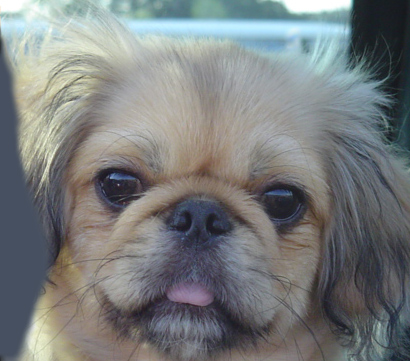
\includegraphics[width=\linewidth]{images/dog.jpg}
          \caption{Dog}
          \label{fig:dog}
      \end{subfigure}
      \quad \quad
      \begin{subfigure}[b]{0.4\textwidth}
          \centering
          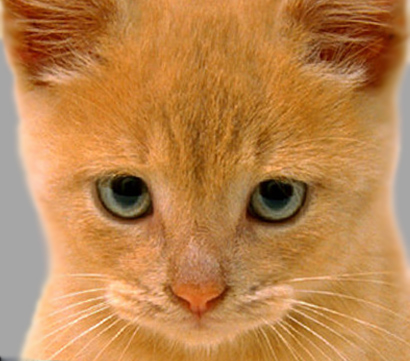
\includegraphics[width=\linewidth]{images/cat.jpg}
          \caption{Cat}
          \label{fig:cat}
      \end{subfigure}
      \caption{}
      \label{fig:dog-cat}
\end{figure}

\noindent
The low-pass (blurred) and high-pass version of these images look like this:

 \begin{figure}[ht]
      \centering
      \begin{subfigure}[b]{0.4\textwidth}
          \centering
          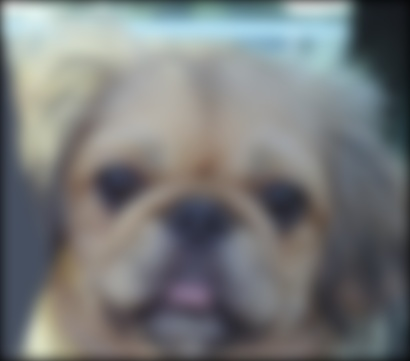
\includegraphics[width=\linewidth]{images/low_frequencies.jpg}
          \caption{Low frequencies of dog image.}
          \label{fig:low}
      \end{subfigure}
      \quad \quad
      \begin{subfigure}[b]{0.4\textwidth}
          \centering
          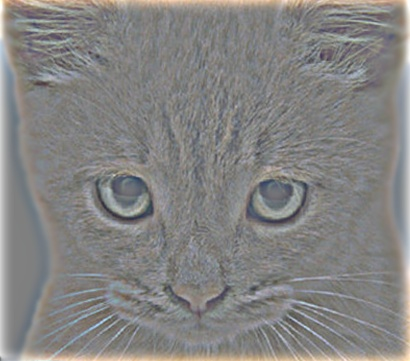
\includegraphics[width=\linewidth]{images/high_frequencies.jpg}
          \caption{High frequencies of cat image.}
          \label{fig:high}
      \end{subfigure}
      \caption{}
      \label{fig:low-high}
\end{figure}

\noindent
The high frequency image in Figure \ref{fig:high} is actually zero-mean with negative values, so it is visualized by adding 0.5. In the resulting visualization, bright values are positive and dark values are negative.
\\
\\
Adding the high and low frequencies together (Figures \ref{fig:high} and \ref{fig:low}, respectively) gives you the image in Figure \ref{fig:hybrid}. If you're having trouble seeing the multiple interpretations of the image, a useful way to visualize the effect is by progressively downsampling the hybrid image, as done in Figure \ref{fig:scales}. The starter code provides a function, \lstinline{vis_image_scales_numpy()} in \lstinline{utils.py}, which can be used to save and display such visualizations.

\begin{figure}[ht]
    \centering
    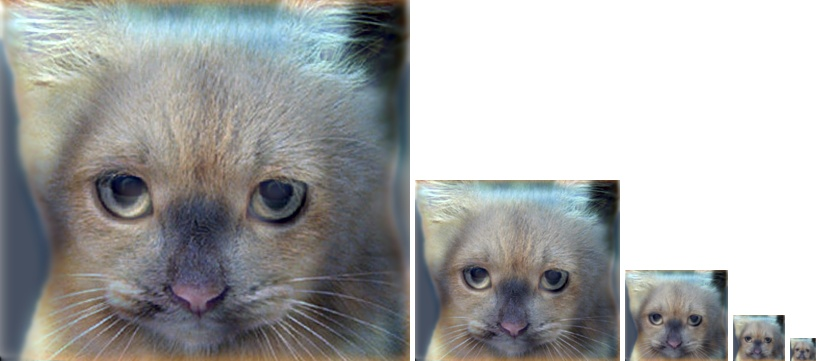
\includegraphics[width=0.75\textwidth]{images/cat_hybrid_image_scales.jpg}
    \caption{}
    \label{fig:scales}
\end{figure}

\subsection*{Potentially useful NumPy (Python library) functions}
\lstinline{np.pad()}, which does many kinds of image padding for you, \lstinline{np.clip()}, which ``clips'' out any values in an array outside of a specified range, \lstinline{np.sum()} and \lstinline{np.multiply()}, which makes it efficient to do the convolution (dot product) between the filter and windows of the image, \lstinline{np.linalg.svd()}, which helps you calculate SVD easily. Documentation for NumPy can be found \href{https://docs.scipy.org/doc/numpy/}{here} or by Googling the function in question.

\subsection*{Forbidden functions}
(You can use these for testing, but not in your final code). Anything that takes care of the filter operation or creates a 2D Gaussian kernel directly for you is forbidden. If it feels like you're sidestepping the work, then it's probably not allowed. Ask the TAs if you have any doubts.

\section*{Testing}
We have provided a set of tests for you to evaluate your implementation. We have included tests inside \lstinline{project-1.ipynb} so you can check your progress as you implement each section. When you're done with the entire project, you can call additional tests by running \lstinline{pytest tests} inside the root directory of the project, as well as checking against the tests on Gradescope. \textit{Your grade on the coding portion of the project will be further evaluated with a set of tests not provided to you.}

\section*{Extra Credit}
For this first assignment, we don't have extra credit. But there will be extra credits available for future assignments. More details will be released.


\section*{Submission}

This is very important as you will lose 5 points for every time you do not follow the instructions. You will submit two items to Gradescope:
\begin{enumerate}
    \item \lstinline{<your_gt_username>.zip} containing:
    \begin{itemize}
        \item \lstinline{src/}: directory containing all your code for this assignment
        \item \lstinline{cutoff_frequency.txt}: .txt file containing the best cutoff frequency values you found for each pair of images in \lstinline{data/}
        \item \lstinline{setup.cfg}: setup file for environment, no need to change this file
        \item \lstinline{additional_data/}: (optional) if you use any data other than the images we provide, please include them here
        \item \lstinline{README.txt}: (optional) if you implement any new functions other than the ones we define in the skeleton code (e.g., any helper function implementations), please describe what you did and how we can run the code
    \end{itemize}
    \item \lstinline{<your_gt_usernamme>_proj1.pdf} - your report
\end{enumerate}


% Do \textbf{\textit{not}} install any additional packages inside the conda environment.
% The TAs will use the same environment as defined in the config files we provide you, so anything that's not in there by default will probably cause your code to break during grading. Do \textbf{\textit{not}} use absolute paths in your code or your code will break. Use relative paths like the starter code already does.
% Failure to follow any of these instructions will lead to point deductions. Create the zip file by clicking and hand it in with your report PDF through Gradescope (please remember to mark which parts of your report correspond to each part of the rubric).


\section*{Credits}
This assignment was developed by Humphrey Shi, Dhruv Patel, Jinghao Miao, Aditya Kane and Manushree Vasu, based on similar projects by James Hays and Judy Hoffman.

\end{document}
